\documentclass[tikz,border=4pt]{standalone}
\usepackage{amsmath}
\begin{document}
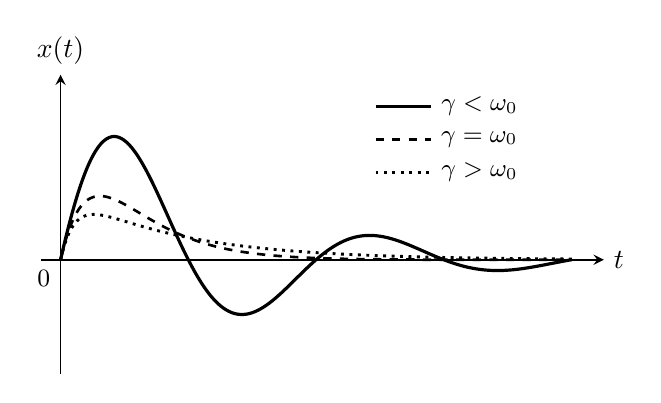
\begin{tikzpicture}[>=stealth, thick, scale=1.0]
  % Axes: t from 0 to 6.8 (scale: omega_0 t = 2.0 * x -> x = 0..6.5 covers omega_0 t = 0..13)
  \draw[->, line width=0.65pt] (-0.25, 0) -- (6.9, 0) node[right] {$t$};
  \draw[->, line width=0.65pt] (0, -1.45) -- (0, 2.35) node[above] {$x(t)$};
  \node[below left, font=\small] at (0, 0) {$0$};

  % Normalize p_0 / (m omega_0) = 2.2 cm
  % Underdamped: gamma / omega_0 = 0.25, Omega/omega_0 = sqrt(1 - 0.0625) = 0.96825
  \draw[line width=1.15pt, domain=0:6.5, samples=180, smooth]
    plot (\x, {2.2 / 0.96825 * exp(-0.25 * 2*\x) * sin(deg(0.96825 * 2*\x))});

  % Critical damping: gamma = omega_0 -> 2.2 * (2x) * exp(-2x)
  \draw[dashed, line width=0.95pt, domain=0:6.5, samples=140, smooth]
    plot (\x, {2.2 * (2*\x) * exp(-2*\x)});

  % Overdamped: gamma / omega_0 = 1.6, Gamma/omega_0 = sqrt(2.56 - 1) = 1.249
  \draw[dotted, line width=1.05pt, domain=0:6.5, samples=140, smooth]
    plot (\x, {2.2 / (2*1.249) * (exp((-1.6+1.249)*2*\x) - exp((-1.6-1.249)*2*\x))});

  % Legend in upper right
  \begin{scope}[xshift=4.0cm, yshift=1.95cm]
    \draw[line width=1.15pt] (0, 0) -- (0.7, 0) node[right, font=\small] {$\gamma < \omega_0$};
    \draw[dashed, line width=0.95pt] (0, -0.42) -- (0.7, -0.42) node[right, font=\small] {$\gamma = \omega_0$};
    \draw[dotted, line width=1.05pt] (0, -0.84) -- (0.7, -0.84) node[right, font=\small] {$\gamma > \omega_0$};
  \end{scope}
\end{tikzpicture}
\end{document}
